% !TEX root=SysSpec_ClockPendulumAnalyzer
\subsection{Umsetzung des GPIO Zugriff}
Der Zugriff auf die GPIO Pins des \rpi\ wurde mit einer simplen Klasse umgesetzt. Diese Klasse ist verantwortlich für das Exportieren und Unexportieren der Pins.
Dies geschieht bei der Initialisierung der Klasse beziehungsweise beim Dekonstruktor. Dabei wird das Prinzip der ''Resourcenbelegung ist Initialisierung'' (kurz RAII) nicht verletzt.\\
\\
Die Aufgaben des Benutzers sind nur Richtung setzen und dann Lesen bzw. Schreiben der Pins. Die Richtung (Output / Input) kann zur Laufzeit geändert werden.

\subsubsection{Pinbelegung}
Die Pinbelegung auf dem \rpi\ sieht wie folgt aus.
\begin{figure}[H]
    \centering
    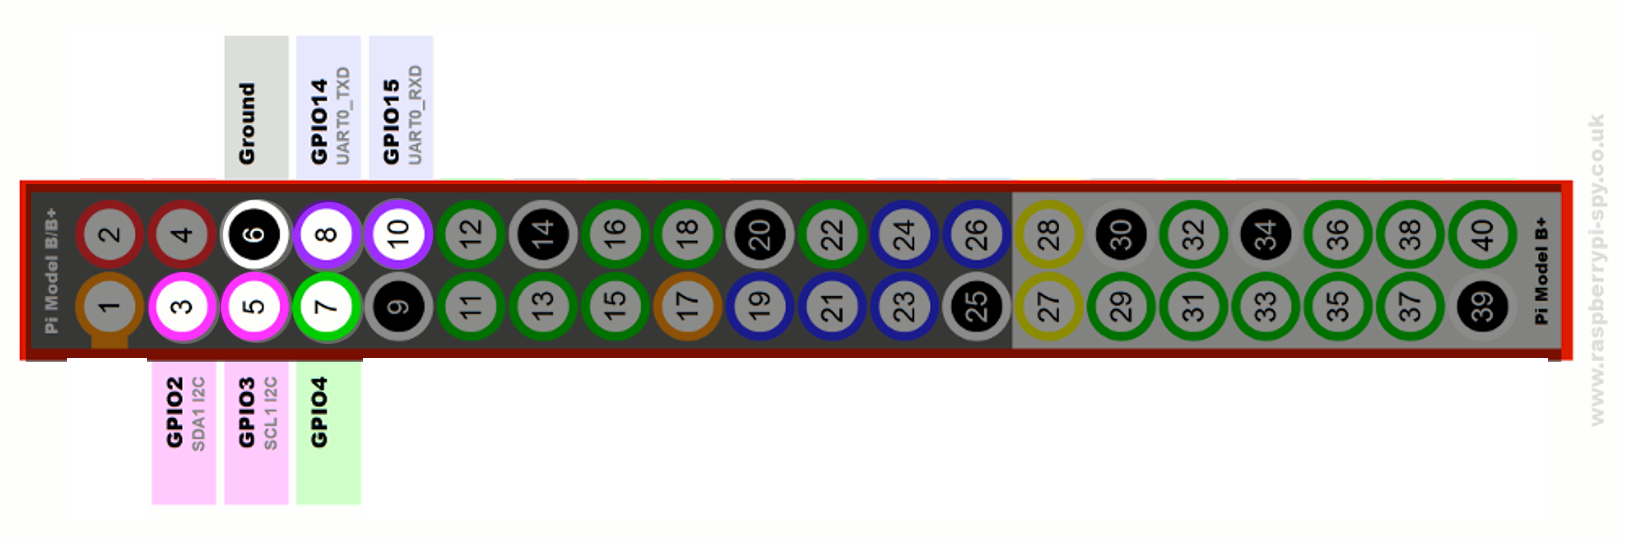
\includegraphics[width=\textwidth]{pinbelegung}
    \caption{Pinbelegung des \rpi\ (Originalbild von www.raspberrypi-spy.co.uk)}
\end{figure}

\noindent Pin 6,8,10,3 und 5 werden nicht durch die GPIO\footnote{General Purpose Input Output} Klasse angesteuert. Diese sind für die UART beziehungsweise \iic\ Kommunikation reserviert, die in den nachfolgenden Kapitel \ref{sec:i2c} und \ref{sec:uart} beschrieben sind.\\\\
Pin 7 dient als Interrupt-Pin für den Hardware Counter. Dieser wird bei Programmstart als High Output Pin gesetzt um damit den Counter zurückzusetzen. Damit wird erreicht, dass das System auf unterschiedliche Aufstartzeiten reagieren kann und die ganze Messung gleichzeitig starten kann. Der Counter-Reset wird nur bei Programmstart ausgeführt und danach nicht mehr.

\subsubsection{\iic\ Implementierung}\label{sec:i2c}
Der \iic\ Anschluss läuft über Pin 3 (SDA\footnote{Data Signal}) und 5 (SCL\footnote{Clock Signal}).\\
Für den \iic\ wurde ebenfalls eine abstrahierende Klasse entwickelt. Diese verwendet die bereits vom Linux bereitgestellten Funktionalitäten zum Lesen und Schreiben von \iic-Geräten.\\
\\
Im Kontext des Clock Pendulum Analyzers ist der \iic\ Bus als Kommunikation zwischen RTC, Counter und \rpi\ gedacht. 
Dabei wäre das \rpi\ der Master und fordert die anderen zwei Teilnehmer nach ihren Daten.

\paragraph{Aufgetretene Probleme:}
Aufgrund des gewählten Betriebssystem und der dadurch entstandenen Problematik mit der Schnittstelle auf dem \rpi, wird die \iic\ Implementierung nicht beendet.\\
Die Problematik bestand darin, dass die \iic-Geräte auf dem Linux nicht erkannt wurden. Nach mehreren Versuchen die Geräte zu erkennen, wurde entschieden, dass zur Kommunikation eine USB-UART Verbindung aufgebaut wird. Diese Verbindung beinhaltet nur noch die Kommunikation mit dem Counterboard. Mehr zum UART ist im folgenden Kapitel \ref{sec:uart} zu lesen.

\clearpage
\subsubsection{UART Implementierung}\label{sec:uart}%TODO rework chapter UART
Für das Lesen des GPS Signals wird eine UART Kommunikation benötigt.
Aufgrund der \iic\ Problematik wird die GPS UART Verbindung auf den zwei Pins 8 und 10 nicht weiter verfolgt.\\
\\
Dafür wird eine USB-UART Verbindung zum Counterboard realisiert. Als Übertragungsmedium dient ein micro-USB Kabel und lässt daher nur eine 1-zu-1 Verbindung zu.\\
\\
Der Code basiert auf einer bereits implementierten Lösung aus einem früheren Projekt und wird auf die Bedürfnisses dieser Kommunikation angepasst.\\
Das Lesen des UARTs findet in einem eigenen Thread auf dem \rpi\ statt und empfängt Signale, die vom Counterboard gesendet werden. Wenn eine Nachricht empfangen wird, wird diese an einer Liste angehängt. Nebenbei läuft der Main-Thread und liest, wenn die Liste einen Eintrag enthält, den Zeitstempel und dessen absolute Zeit aus. Danach wird dieser Eintrag aus der Liste entfernt.